\documentclass[border=5pt]{standalone}

% Required for Bengali text rendering
\usepackage{fontspec}
\usepackage{amsmath}
\usepackage{tikz}

\setmainfont{Noto Sans Bengali}

\begin{document}

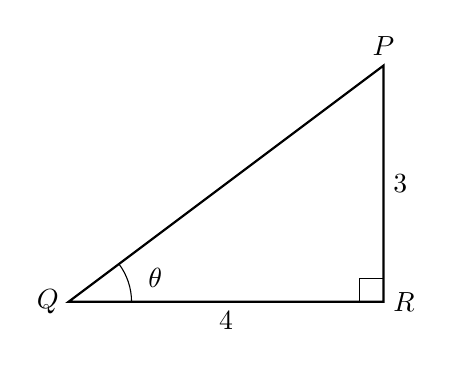
\begin{tikzpicture}[scale=1]
    % Coordinates for the right-angled triangle PQR
    \coordinate (Q) at (0,0);
    \coordinate (R) at (4,0);
    \coordinate (P) at (4,3);

    % Draw the triangle
    \draw[thick] (Q) -- (R) -- (P) -- cycle;

    % Draw the right-angle symbol at R
    \draw (3.7,0) -- (3.7,0.3) -- (4,0.3);

    % Draw the angle arc for theta at Q
    \draw (0.8,0) arc (0:36.87:0.8);
    \node at (1.1,0.3) {$\theta$};

    % Label the points exactly as shown in the image
    \node[left] at (Q) {$Q$};
    \node[right] at (R) {$R$};
    \node[above] at (P) {$P$};

    % Add the measurements exactly as they appear
    \node[below] at (2,0) {$4$};
    \node[right] at (4,1.5) {$3$};

\end{tikzpicture}

\end{document}
